\whiteBGstarBegin
\setcounter{section}{0}
\section{Lý thuyết: Năng lượng liên kết, năng lượng liên kết riêng của hạt nhân}
\begin{enumerate}[label=\bfseries Câu \arabic*:]
	\item \mkstar{1} [1]
	
	\cauhoi
	{Đại lượng đặc trưng cho mức độ bền vững của hạt nhân là
		\begin{mcq}(2)
			\item độ hụt khối.
			\item năng lượng liên kết.
			\item khối lượng hạt nhân.
			\item năng lượng liên kết riêng.
		\end{mcq}
	}
	
	\loigiai
	{		\textbf{Đáp án: D.}
		
		Đại lượng đặc trưng cho mức độ bền vững của hạt nhân là năng lượng liên kết riêng. Năng lượng liên kết riêng càng lớn thì hạt nhân càng bền vững và ngược lại.
		
	}
		\item \mkstar{1} [2]
	
	\cauhoi
	{Tìm phát biểu \textbf{sai} khi nói về độ hụt khối.
		\begin{mcq}
			\item Độ hụt khối của một hạt nhân thường khác không nhưng trong trường hợp đặc biệt thì cũng có thể bằng không. 
			\item Độ chênh lệch giữa khối lượng $m$ của hạt nhân và tổng khối lượng $m_0$ của các nuclon cấu tạo nên hạt nhân gọi là độ hụt khối.
			\item Khối lượng của một hạt nhân luôn nhỏ hơn tổng khối lượng của các nuclon cấu tạo thành hạt nhân đó. 
			\item Khối lượng của một hạt nhân luôn lớn hơn tổng khối lượng của các nuclon cấu tạo thành hạt nhân đó.
		\end{mcq}
	}
	
	\loigiai
	{		\textbf{Đáp án: D.}
		
		"Khối lượng của một hạt nhân luôn lớn hơn tổng khối lượng của các nuclon cấu tạo thành hạt nhân đó." là phát biểu sai.
		
		"Khối lượng của một hạt nhân luôn nhỏ hơn tổng khối lượng của các nuclon cấu tạo thành hạt nhân đó." là phát biểu đúng.
		
	}
	\item \mkstar{1} [3]

\cauhoi
{Hạt nhân có năng lượng liên kết càng lớn thì
	\begin{mcq}(2)
		\item càng kém bền vững.
		\item độ hụt khối của hạt nhân càng nhỏ.
		\item độ hụt khối của hạt nhân càng lớn.
		\item càng bền vững.
	\end{mcq}
}

\loigiai
{		\textbf{Đáp án: C.}
	
	Hạt nhân có năng lượng liên kết càng lớn thì độ hụt khối của hạt nhân càng lớn:
	$$E_\text{lk} = \Delta m c^2$$
	
}
\item \mkstar{1} [4]

\cauhoi
{Đại lượng nào sau đây đặc trưng cho mức độ bền vững của hạt nhân?
	\begin{mcq}(2)
		\item Năng lượng nghỉ.
		\item Độ hụt khối.
		\item Năng lượng liên kết.
		\item Năng lượng liên kết riêng.
	\end{mcq}
}

\loigiai
{		\textbf{Đáp án: D.}
	
	Đại lượng đặc trưng cho mức độ bền vững của hạt nhân là năng lượng liên kết riêng. Năng lượng liên kết riêng càng lớn thì hạt nhân càng bền vững và ngược lại.
	
	
}
\item \mkstar{1} [5]

\cauhoi
{Để so sánh độ bền vững của các hạt nhân người ta thường dùng đại lượng:
	\begin{mcq}
		\item năng lượng liên kết tính trên một nuclon.
		\item năng lượng liên kết tính cho một hạt nhân.
		\item năng lượng liên kết giữa hai nuclon.
		\item năng lượng liên kết giữa hạt nhân và lớp vỏ nguyên tử.
	\end{mcq}
}

\loigiai
{		\textbf{Đáp án: A.}
	
	Để so sánh độ bền vững của các hạt nhân người ta thường dùng năng lượng liên kết riêng: năng lượng liên kết tính trên một nuclon.
	
}
\item \mkstar{1} [5]

\cauhoi
{Năng lượng liên kết riêng là năng lượng liên kết ...
	\begin{mcq}(2)
		\item tính riêng cho hạt nhân ấy.
		\item tính cho một nuclon.
		\item của một cặp proton - proton.
		\item của một cặp proton - nơtron.
	\end{mcq}
}

\loigiai
{		\textbf{Đáp án: B.}
	
	Năng lượng liên kết riêng là năng lượng liên kết tính cho một nuclon.
	
}
\item \mkstar{1} [7]

\cauhoi
{Năng lượng liên kết riêng của một hạt nhân
	\begin{mcq}(2)
		\item có thể âm hoặc dương.
		\item càng lớn, thì càng kém bền vững.
		\item càng nhỏ, thì càng bền vững.
		\item càng lớn, thì càng bền vững.
	\end{mcq}
}

\loigiai
{		\textbf{Đáp án: D.}
	
	Năng lượng liên kết riêng của một hạt nhân càng lớn thì hạt nhân đó càng bền vững.
	
}
\item \mkstar{1} [9]

\cauhoi
{Hạt nhân càng bền vững khi có
	\begin{mcq}(2)
		\item năng lượng liên kết càng lớn.
		\item số nuclon càng nhỏ.
		\item số nuclon càng lớn.
		\item năng lượng liên kết riêng càng lớn.
	\end{mcq}
}

\loigiai
{		\textbf{Đáp án: D.}
	
	Càng nhân càng bền vững khi có năng lượng liên kết riêng càng lớn.
	
}
	\item \mkstar{2} [1]
	
	\cauhoi
	{Độ hụt khối khi hình thành hạt nhân $\ce{^12_6 C}$ bằng $\SI{89.424}{MeV/c^2}$. Năng lượng liên kết riêng của hạt nhân này bằng
		\begin{mcq}(4)
			\item $\SI{7.452}{MeV}$.
			\item $\SI{6.387}{MeV}$.
			\item $\SI{6.837}{MeV}$.
			\item $\SI{7.542}{MeV}$.
		\end{mcq}
	}
	
	\loigiai
	{		\textbf{Đáp án: A.}
		
		Năng lượng liên kết:
		$$E_\text{lk} = \Delta m c^2 = \SI{89.424}{MeV/c^2} \cdot c^2 = \SI{89.424}{MeV}$$
		
		Năng lượng liên kết riêng:
		$$E_\text{lkr} = \dfrac{E_\text{lk}}{A} = \SI{7.452}{MeV}$$
		
	}
	
	\item \mkstar{2} [1]
	
	\cauhoi
	{Hạt nhân đơteri $\ce{^2_1 D}$ có năng lượng liên kết là $\SI{2.23}{MeV}$. Biết khối lượng của proton là $\SI{1.0073}{u}$ và khối lượng của nơtron là $\SI{1.0087}{u}$. Hạt nhân $\ce{^2_1 D}$ có khối lượng là
		\begin{mcq}(4)
			\item $\SI{2.1036}{u}$. 
			\item $\SI{2.0136}{u}$. 
			\item $\SI{2.1360}{u}$. 
			\item $\SI{2.0361}{u}$. 
		\end{mcq}
	}
	
	\loigiai
	{		\textbf{Đáp án: B.}
		
		Độ hụt khối của hạt nhân:
		$$E_\text{lk} = \Delta m c^2 \Rightarrow \Delta m = \dfrac{E_\text{lk}}{c^2} = \dfrac{2,23}{931,5} = \SI{2.4e-3}{u}$$
		
		Khối lượng hạt nhân $\ce{^2_1 D}$:
		$$\Delta m = Zm_p + (A-Z)m_n - m_X \Rightarrow m_X = \SI{2.0136}{u}$$
	}
	

	
	\item \mkstar{2} [2]
	
	\cauhoi
	{Hạt nhân đơ-tơ-ri $\ce{^2_1 D}$ có khối lượng $\SI{2.0136}{u}$. Biết khối lượng của proton là $\SI{1.0073}{u}$ và khối lượng của nơtron là $\SI{1.0087}{u}$. Lấy $\SI{1}{u}=\SI{931.5}{MeV/c^2}$. Năng lượng liên kết riêng của hạt nhân $\ce{^2_1 D}$ là
		\begin{mcq}(2)
			\item $\SI{1.1178}{MeV/nuclon}$. 
			\item $\SI{2.2356}{MeV/nuclon}$. 
			\item $\SI{0.6753}{MeV/nuclon}$.
			\item $\SI{2.0218}{MeV/nuclon}$.
		\end{mcq}
	}
	
	\loigiai
	{		\textbf{Đáp án: A.}
		
		Độ hụt khối:
		$$\Delta m = Zm_p + (A-Z)m_n - m_X = \SI{2.4e-3}{u}$$
		
		Năng lượng liên kết:
		$$E_\text{lk} = \Delta m c^2 = \SI{2.2356}{MeV}$$
		
		Năng lượng liên kết riêng:
		$$E_\text{lkr} = \dfrac{E_\text{lk}}{A} =\SI{1.1178}{MeV/nuclon} $$
		
	}

\item \mkstar{2} [3]

\cauhoi
{Hạt nhân đơ-tơ-ri $\ce{^2_1 D}$ có khối lượng $\SI{2.0136}{u}$. Biết khối lượng của proton là $\SI{1.0073}{u}$ và khối lượng của nơtron là $\SI{1.0087}{u}$. Lấy $\SI{1}{u}=\SI{931.5}{MeV/c^2}$. Năng lượng liên kết của hạt nhân $\ce{^2_1 D}$ là
	\begin{mcq}(4)
		\item $\SI{3.06}{MeV}$. 
		\item $\SI{1.12}{MeV}$. 
		\item $\SI{4.48}{MeV}$.
		\item $\SI{2.24}{MeV}$.
	\end{mcq}
}

\loigiai
{		\textbf{Đáp án: D.}
	
	Độ hụt khối:
	$$\Delta m = Zm_p + (A-Z)m_n - m_X = \SI{2.4e-3}{u}$$
	
	Năng lượng liên kết:
	$$E_\text{lk} = \Delta m c^2 = \SI{2.24}{MeV}$$
	
}
\item \mkstar{2} [2]

\cauhoi
{Hạt nhân $\ce{^37_17 Cl}$ có khối lượng nghỉ bằng $\SI{36.956563}{u}$. Biết khối lượng của nơtron là $\SI{1.008670}{u}$, khối lượng của proton là $\SI{1.007276}{}$ và $\SI{1}{u} = \SI{931.5}{MeV/c^2}$. Năng lượng liên kết riêng của hạt nhân $\ce{^37_17 Cl}$ bằng
	\begin{mcq}(4)
		\item $\SI{6.325}{MeV}$.
		\item $\SI{7.368}{MeV}$.
		\item $\SI{8.468}{MeV}$.
		\item $\SI{8.573}{MeV}$.
	\end{mcq}
}

\loigiai
{		\textbf{Đáp án: D.}
	
		Độ hụt khối:
	$$\Delta m = Zm_p + (A-Z)m_n - m_X = \SI{0.340529}{u}$$
	
	Năng lượng liên kết:
	$$E_\text{lk} = \Delta m c^2 = \SI{317.2028}{MeV}$$
	
	Năng lượng liên kết riêng:
	$$E_\text{lkr} = \dfrac{E_\text{lk}}{A} =\SI{8.573}{MeV/nuclon} $$
	
}

\item \mkstar{2} [4]

\cauhoi
{Biết khối lượng của hạt nhân $\ce{^235_92 U}$ là $\SI{234.99}{u}$, của proton là $\SI{1.0073}{u}$ và của nơtron là $\SI{1.0087}{u}$. Năng lượng liên kết riêng của hạt nhân $\ce{^235_92 U}$ là
	\begin{mcq}(2)
		\item $\SI{7.95}{MeV/nuclon}$.
		\item $\SI{6.73}{MeV/nuclon}$.
		\item $\SI{8.71}{MeV/nuclon}$.
		\item $\SI{7.63}{MeV/nuclon}$.
	\end{mcq}
}

\loigiai
{		\textbf{Đáp án: D.}
	
		Độ hụt khối:
	$$\Delta m = Zm_p + (A-Z)m_n - m_X = \SI{1.9257}{u}$$
	
	Năng lượng liên kết:
	$$E_\text{lk} = \Delta m c^2 = \SI{1793.79}{MeV}$$
	
	Năng lượng liên kết riêng:
	$$E_\text{lkr} = \dfrac{E_\text{lk}}{A} =\SI{7.63}{MeV/nuclon} $$
	
}

\item \mkstar{2} [12]

\cauhoi
{Biết năng lượng liên kết của hạt nhân $\ce{^7_3 Li}$ là $\SI{62.40}{MeV}$. Năng lượng liên kết riêng của nó xấp xỉ bằng
	\begin{mcq}(4)
		\item $\SI{20.80}{MeV/nuclon}$.
		\item $\SI{4.455}{MeV/nuclon}$.
		\item $\SI{10.40}{MeV/nuclon}$.
		\item $\SI{8.910}{MeV/nuclon}$.
	\end{mcq}
}

\loigiai
{		\textbf{Đáp án: D.}
	
	Năng lượng liên kết riêng:
	$$E_\text{lkr} = \dfrac{E_\text{lk}}{A} \approx \SI{8.910}{MeV/nuclon} $$
	
}



\item \mkstar{2} [5]

\cauhoi
{Hạt nhân Côban $\ce{^60_27 Co}$ có khối lượng $m_{\ce{Co}} = \SI{55.940}{u}$. Biết khối lượng của proton là $m_p=\SI{1.0073}{u}$ và khối lượng của nơtron là $m_n=\SI{1.0087}{u}$. Năng lượng liên kết riêng của hạt nhân $\ce{^60_27 Co}$ là
	\begin{mcq}(2)
		\item $\SI{48.9}{MeV/nuclon}$.
		\item $\SI{54.4}{MeV/nuclon}$.
		\item $\SI{70.4}{MeV/nuclon}$.
		\item $\SI{70.5}{MeV/nuclon}$.
	\end{mcq}
}

\loigiai
{		\textbf{Đáp án: D.}
	
	Độ hụt khối:
	$$\Delta m = Zm_p + (A-Z)m_n - m_X = \SI{4.5442}{u}$$
	
	Năng lượng liên kết:
	$$E_\text{lk} = \Delta m c^2 = \SI{4232.9223}{MeV}$$
	
	Năng lượng liên kết riêng:
	$$E_\text{lkr} = \dfrac{E_\text{lk}}{A} =\SI{70.5}{MeV/nuclon} $$
	
}

\item \mkstar{2} [7]

\cauhoi
{Một hạt nhân $\ce{^4_2 He}$ có độ hụt khối là $\SI{0.0305}{u}$. Lấy $\SI{1}{u} = \SI{931.5}{MeV/c^2}$. Năng lượng liên kết riêng của hạt nhân này là
	\begin{mcq}(2)
		\item $\SI{28.41075}{MeV/nuclon}$.
		\item $\SI{7.10269}{eV/nuclon}$.
		\item $\SI{7.10269}{MeV/nuclon}$.
		\item $\SI{7.01269}{MeV/nuclon}$.
	\end{mcq}
}

\loigiai
{		\textbf{Đáp án: C.}
	
	
	Năng lượng liên kết:
	$$E_\text{lk} = \Delta m c^2 = \SI{28.41075}{MeV}$$
	
	Năng lượng liên kết riêng:
	$$E_\text{lkr} = \dfrac{E_\text{lk}}{A} =\SI{7.10269}{MeV/nuclon} $$
}

\item \mkstar{2} [9]

\cauhoi
{Hạt nhân Rađi $\ce{^226_88 Ra}$ có khối lượng bằng $\SI{225.9771}{u}$. Biết khối lượng của nơtron là $\SI{1.00867}{u}$, khối lượng của proton là $\SI{1.00728}{u}$. Năng lượng liên kết riêng của hạt nhân $\ce{^226_88 Ra}$ bằng
	\begin{mcq}(2)
		\item $\SI{1732.59}{MeV/nuclon}$.
		\item $\SI{1667.85}{MeV/nuclon}$.
		\item $\SI{7.67}{MeV/nuclon}$.
		\item $\SI{7.38}{MeV/nuclon}$.
	\end{mcq}
}

\loigiai
{		\textbf{Đáp án: C.}
	
	Độ hụt khối:
	$$\Delta m = Zm_p + (A-Z)m_n - m_X = \SI{1.86}{u}$$
	
	Năng lượng liên kết:
	$$E_\text{lk} = \Delta m c^2 = \SI{1732.59}{MeV}$$
	
	Năng lượng liên kết riêng:
	$$E_\text{lkr} = \dfrac{E_\text{lk}}{A} =\SI{7.67}{MeV/nuclon} $$
	
}
\item \mkstar{3} [9]

\cauhoi
{Hạt nhân $\ce{^4_2 He}$ có năng lượng liên kết riêng là $\SI{7.1}{MeV/nuclon}$. Cho $\SI{1}{u} = \SI{931.5}{MeV/c^2}$. Độ hụt khối của hạt nhân $\ce{^4_2 He}$ là
	\begin{mcq}(4)
		\item $\SI{0.0076}{u}$.
		\item $\SI{0.0305}{u}$.
		\item $\SI{0.751}{u}$.
		\item $\SI{1.917}{u}$.
	\end{mcq}
}

\loigiai
{		\textbf{Đáp án: B.}
	
	Năng lượng liên kết:
	$$E_\text{lk} = E_\text{lkr} A = \SI{28.4}{MeV}$$
	
	Độ hụt khối của hạt nhân:
	$$E_\text{lk} = \Delta m c^2 \Rightarrow \Delta m = \dfrac{E_\text{lk}}{c^2} = \dfrac{28,4}{931,5} = \SI{0.0305}{u}$$
	
}
\item \mkstar{3} [13]

\cauhoi
{Biết khối lượng của nơtron là $\SI{1.00867}{u}$, khối lượng của proton là $\SI{1.00728}{u}$, khối lượng của hạt nhân $\ce{^10_5 B}$ là $\SI{10.0102}{u}$. Năng lượng liên kết riêng của hạt nhân này bằng
	\begin{mcq}(4)
		\item $\SI{5.885}{MeV}$.
		\item $\SI{6.479}{MeV}$.
		\item $\SI{12.948}{MeV}$.
		\item $\SI{64.79}{MeV}$.
	\end{mcq}
}

\loigiai
{		\textbf{Đáp án: B.}
	
	Độ hụt khối:
	$$\Delta m = Zm_p + (A-Z)m_n - m_X = \SI{0.0696}{u}$$
	
	Năng lượng liên kết:
	$$E_\text{lk} = \Delta m c^2 = \SI{64.79}{MeV}$$
	
	Năng lượng liên kết riêng:
	$$E_\text{lkr} = \dfrac{E_\text{lk}}{A} =\SI{6.479}{MeV/nuclon} $$
	
	Vậy $\SI{6.474}{MeV}$ là đáp án gần đúng nhất.
	
}
\end{enumerate}

\loigiai
{
	\begin{center}
		\textbf{BẢNG ĐÁP ÁN}
	\end{center}
	\begin{center}
		\begin{tabular}{|m{2.8em}|m{2.8em}|m{2.8em}|m{2.8em}|m{2.8em}|m{2.8em}|m{2.8em}|m{2.8em}|m{2.8em}|m{2.8em}|}
			\hline
			1.D  & 2.D  & 3.C  & 4.D  & 5.A  & 6.B  & 7.D & 8.D & 9.A & 10.B \\
			\hline
			11.A  & 12.D  & 13.D  & 14.D  & 15.D  & 16.D  & 17.C & 18.C & 19.B & 20.B \\
			\hline
		\end{tabular}
	\end{center}
}

\section{Dạng bài: Phương trình phản ứng hạt nhân. Năng lượng tỏa ra hoặc thu vào trong phản ứng hạt nhân}
\begin{enumerate}[label=\bfseries Câu \arabic*:]
	\item \mkstar{1} [2]
	
	\cauhoi
	{Chọn câu \textbf{sai} khi nói về phản ứng hạt nhân tỏa năng lượng.
		\begin{mcq}
			\item Năng lượng tỏa ra dưới dạng động năng của các hạt tạo thành.
			\item Các hạt tạo thành sau phản ứng bền vững hơn các hạt trước phản ứng.
			\item Tổng độ hụt khối của các hạt trước phản ứng lớn hơn tổng độ hụt khối của các hạt sau phản ứng.
			\item Tổng khối lượng các hạt trước phản ứng lớn hơn tổng khối lượng các hạt sau phản ứng.
		\end{mcq}
	}
	
	\loigiai
	{		\textbf{Đáp án: C.}
		
		Trong phản ứng hạt nhân tỏa năng lượng, tổng khối lượng các hạt trước phản ứng lớn hơn tổng khối lượng các hạt sau phản ứng, các hạt tạo thành sau phản ứng bền vững hơn các hạt trước phản ứng, năng lượng tỏa ra dưới dạng động năng của các hạt tạo thành.
		
		Trong phản ứng hạt nhân tỏa năng lượng, tổng độ hụt khối của các hạt trước phản ứng nhỏ hơn tổng độ hụt khối của các hạt sau phản ứng.
		
	}
	\item \mkstar{2} [4]
	
	\cauhoi
	{Cho phản ứng hạt nhân sau: $\ce{^1_1 H} + \ce{^9_4 Be} \longrightarrow \ce{^4_2 He} + \ce{^7_3 Li} + \SI{2.1}{MeV}$. Năng lượng tỏa ra từ phản ứng trên khi tổng hợp được $\SI{0.5}{mol}$ He là
		\begin{mcq}(4)
			\item $\SI{12.642e23}{MeV}$.
			\item $\SI{6.321e21}{MeV}$.
			\item $\SI{12.642e21}{MeV}$.
			\item $\SI{6.321e23}{MeV}$.
		\end{mcq}
	}
	
	\loigiai
	{		\textbf{Đáp án: D.}
		
		Số hạt nhân He có trong $\SI{0.5}{mol}$ là
		$$N=0,5 \cdot N_\text{A} = \SI{3.011e23}{}$$
		
		Mỗi phản ứng tỏa ra năng lượng là $\SI{2.1}{MeV}$, vậy năng lượng tỏa ra từ $\SI{3.011e23}{}$ phản ứng là
		$$\SI{3.011e23}{} \cdot \SI{2.1}{MeV} = \SI{6.321e23}{MeV}$$
		
	}
	\item \mkstar{2} [1]
	
	\cauhoi
	{Cho phản ứng hạt nhân $\ce{^235_92 U} + \ce{^1_0 n} \longrightarrow \ce{^95_42 Mo} + \ce{X} + 2\ce{^1_0 n} + 4\ce{^0_{-1} e}$, trong đó X là hạt nhân
		\begin{mcq}(4)
			\item $\ce{^138_53 I}$.
			\item $\ce{^138_52 Te}$.
			\item $\ce{^139_54 Xe}$.
			\item $\ce{^139_57 La}$.
		\end{mcq}
	}
	
	\loigiai
	{		\textbf{Đáp án: C.}
		
		Số khối trước phản ứng: $A_\text{t} = 236$.
		
		Số khối sau phản ứng phải bằng số khối trước phản ứng:
		$$A_\text{s} = A_\text{t} \Rightarrow 95+A_\text X+2\cdot 2 + 4 \cdot 0 = 236 \Rightarrow A_\text X = 139$$
		
		Số điện tích trước phản ứng: $Z_\text{t} = 92$.
		
		Số điện tích sau phản ứng phải bằng số điện tích trước phản ứng:
		$$Z_\text{s} = Z_\text{t} \Rightarrow 42 + Z_\text{X} + 2 \cdot 0 + 4 \cdot(-1) = 92 \Rightarrow Z_\text{X} = 54$$
		
		Vậy X là hạt nhân $\ce{^139_54 Xe}$.
		
	}
	
	\item \mkstar{2} [4]
	
	\cauhoi
	{Trong phản ứng hạt nhân $\ce{^19_9 F} + \ce{p} \longrightarrow \ce{^16_8 O} + \ce{X}$, hạt X là
		\begin{mcq}(4)
			\item nơtron. 
			\item proton. 
			\item hạt $\ce{^4_2 He}$. 
			\item electron.
		\end{mcq}
	}
	
	\loigiai
	{		\textbf{Đáp án: C.}
		
			Số khối trước phản ứng: $A_\text{t} = 20$.
		
		Số khối sau phản ứng phải bằng số khối trước phản ứng:
		$$A_\text{s} = A_\text{t} \Rightarrow 16+A_\text X = 20 \Rightarrow A_\text X = 4$$
		
		Số điện tích trước phản ứng: $Z_\text{t} = 10$.
		
		Số điện tích sau phản ứng phải bằng số điện tích trước phản ứng:
		$$Z_\text{s} = Z_\text{t} \Rightarrow 8 + Z_\text{X} = 10 \Rightarrow Z_\text{X} = 2$$
		
		Vậy X là hạt nhân $\ce{^4_2 He}$.
		
	}
	
	
	
	\item \mkstar{2} [12]
	
	\cauhoi
	{Trong phản ứng hạt nhân $\ce{^35_17 Cl} + \ce{X} \longrightarrow \ce{^32_16 S} + \ce{^4_2 He}$, hạt X là
		\begin{mcq}(4)
			\item $\ce{^2_1 H}$.
			\item $\ce{^3_1 H}$. 
			\item $\ce{^1_1 H}$. 
			\item $\ce{^1_0 n}$.
		\end{mcq}
	}
	
	\loigiai
	{		\textbf{Đáp án: C.}
		
		Số khối sau phản ứng: $A_\text{s} = 36$.
		
		Số khối sau phản ứng phải bằng số khối trước phản ứng:
		$$A_\text{t} = A_\text{s} \Rightarrow 35+A_\text X = 36 \Rightarrow A_\text X = 1$$
		
		Số điện tích sau phản ứng: $Z_\text{s} = 18$.
		
		Số điện tích sau phản ứng phải bằng số điện tích trước phản ứng:
		$$Z_\text{t} = Z_\text{s} \Rightarrow 17 + Z_\text{X} = 18 \Rightarrow Z_\text{X} = 1$$
		
		Vậy X là hạt nhân $\ce{^1_1 H}$.
		
	}
	\item \mkstar{2} [13]
	
	\cauhoi
	{Trong phản ứng hạt nhân $\ce{^9_4 Be} + \ce{\alpha} \longrightarrow \ce{X} + \ce{n}$, hạt X là
		\begin{mcq}(4)
			\item $\ce{^13_7 N}$.
			\item $\ce{^12_6 C}$.
			\item $\ce{^12_5 B}$. 
			\item $\ce{^16_8 O}$.
		\end{mcq}
	}
	
	\loigiai
	{		\textbf{Đáp án: B.}
		
		Số khối trước phản ứng: $A_\text{t} = 13$.
		
		Số khối sau phản ứng phải bằng số khối trước phản ứng:
		$$A_\text{s} = A_\text{t} \Rightarrow 1+A_\text X = 13 \Rightarrow A_\text X = 12$$
		
		Số điện tích trước phản ứng: $Z_\text{t} = 6$.
		
		Số điện tích sau phản ứng phải bằng số điện tích trước phản ứng:
		$$Z_\text{s} = Z_\text{t} \Rightarrow 0 + Z_\text{X} = 6 \Rightarrow Z_\text{X} = 6$$
		
		Vậy X là hạt nhân $\ce{^12_6 C}$.
		
	}
\item \mkstar{2} [5]

\cauhoi
{Trong phản ứng hạt nhân $\ce{^3_1 T} + \ce{X} \longrightarrow \ce{\alpha} + \ce{n}$, hạt X là hạt nhân nào sau đây?
	\begin{mcq}(4)
		\item $\ce{^4_2 He}$. 
		\item $\ce{^2_1 D}$. 
		\item $\ce{^3_1 T}$. . 
		\item $\ce{^1_1 H}$. 
	\end{mcq}
}

\loigiai
{		\textbf{Đáp án: B.}
	
	Số khối sau phản ứng: $A_\text{s} = 5$.
	
	Số khối sau phản ứng phải bằng số khối trước phản ứng:
	$$A_\text{t} = A_\text{s} \Rightarrow 3+A_\text X = 5 \Rightarrow A_\text X = 2$$
	
	Số điện tích sau phản ứng: $Z_\text{s} = 2$.
	
	Số điện tích sau phản ứng phải bằng số điện tích trước phản ứng:
	$$Z_\text{t} = Z_\text{s} \Rightarrow 1 + Z_\text{X} = 2 \Rightarrow Z_\text{X} = 1$$
	
	Vậy X là hạt nhân $\ce{^2_1 D}$.
	
}
\item \mkstar{2} [5]

\cauhoi
{Trong phản ứng hạt nhân $\ce{^37_17 Cl} + \ce{X} \longrightarrow \ce{^37_18 Ar} + \ce{n}$, hạt X là hạt nhân nào sau đây?
	\begin{mcq}(4)
		\item $\ce{^3_1 T}$. 
		\item $\ce{^4_2 He}$. 
		\item $\ce{^2_1 D}$.
		\item $\ce{^1_1 H}$. 
	\end{mcq}
}

\loigiai
{		\textbf{Đáp án: D.}
	
	Số khối sau phản ứng: $A_\text{s} = 38$.
	
	Số khối sau phản ứng phải bằng số khối trước phản ứng:
	$$A_\text{t} = A_\text{s} \Rightarrow 37+A_\text X = 38 \Rightarrow A_\text X = 1$$
	
	Số điện tích sau phản ứng: $Z_\text{s} = 18$.
	
	Số điện tích sau phản ứng phải bằng số điện tích trước phản ứng:
	$$Z_\text{t} = Z_\text{s} \Rightarrow 17 + Z_\text{X} = 18 \Rightarrow Z_\text{X} = 1$$
	
	Vậy X là hạt nhân $\ce{^1_1 H}$.
	
}
\item \mkstar{2} [7]

\cauhoi
{Khi bắn phá hạt nhân $\ce{^14_7 N}$ bằng hạt $\ce{\alpha}$, người ta thu được một hạt proton và một hạt nhân $\ce{X}$. Hạt nhân X là
	\begin{mcq}(4)
		\item $\ce{^17_8 O}$.
		\item $\ce{^16_8 O}$.
		\item $\ce{^12_6 O}$.
		\item $\ce{^14_6 C}$.
	\end{mcq}
}

\loigiai
{		\textbf{Đáp án: A.}
	
	Phương trình phản ứng:
	$$\ce{^14_7 N} + \ce{\alpha} \longrightarrow \ce{p} + \ce{X}$$
	
	Số khối trước phản ứng: $A_\text{t} = 18$.
	
	Số khối sau phản ứng phải bằng số khối trước phản ứng:
	$$A_\text{s} = A_\text{t} \Rightarrow 1+A_\text X = 18 \Rightarrow A_\text X = 17$$
	
	Số điện tích trước phản ứng: $Z_\text{t} = 9$.
	
	Số điện tích sau phản ứng phải bằng số điện tích trước phản ứng:
	$$Z_\text{s} = Z_\text{t} \Rightarrow 1 + Z_\text{X} = 9 \Rightarrow Z_\text{X} = 8$$
	
	Vậy X là hạt nhân $\ce{^17_8 O}$.
	
}
\item \mkstar{2} [9]

\cauhoi
{Trong phản ứng hạt nhân $\ce{\alpha} + \ce{^27_13 Al} \longrightarrow \ce{^30_15 p} + \ce{X}$, hạt X là hạt nhân nào sau đây?
	\begin{mcq}(4)
		\item proton.
		\item electron. 
		\item nơtron. 
		\item pôzitron.
	\end{mcq}
}

\loigiai
{		\textbf{Đáp án: C.}
	
	Số khối trước phản ứng: $A_\text{t} = 31$.
	
	Số khối sau phản ứng phải bằng số khối trước phản ứng:
	$$A_\text{s} = A_\text{t} \Rightarrow 30+A_\text X = 31 \Rightarrow A_\text X = 1$$
	
	Số điện tích trước phản ứng: $Z_\text{t} = 15$.
	
	Số điện tích sau phản ứng phải bằng số điện tích trước phản ứng:
	$$Z_\text{s} = Z_\text{t} \Rightarrow 15 + Z_\text{X} = 15 \Rightarrow Z_\text{X} = 0$$
	
	Vậy X là hạt nhân $\ce{^1_0 n}$.
	
}
\item \mkstar{2} [4]

\cauhoi
{Cho phản ứng hạt nhân $\ce{^4_2 He} + \ce{^27_13 Al} \longrightarrow \ce{^30_15 P} + \ce{n}$, khối lượng của các hạt nhân là $m_{\ce{He}} = \SI{4.0015}{u}$, $m_{\ce{Al}} = \SI{26.97435}{u}$, $m_{\ce{P}} = \SI{29.97005}{u}$, $m_{\ce{n}} = \SI{1.00867}{u}$, $\SI{1}{u} = \SI{931.5}{MeV/c^2}$. Năng lượng mà phản ứng này tỏa ra hoặc thu vào là bao nhiêu?
	\begin{mcq}(2)
		\item Tỏa ra $\SI{5.022648}{MeV}$.
		\item Tỏa ra $\SI{5.022648e-13}{J}$.
		\item Thu vào $\SI{2.673405}{MeV}$.
		\item Thu vào $\SI{2.673405e-13}{J}$.
	\end{mcq}
}

\loigiai
{		\textbf{Đáp án: C.}
	
	Năng lượng tỏa ra hoặc thu vào:
	$$Q=(m_{\text{t}} - m_\text{s}) c^2 = \SI{-2.673405}{MeV}$$
	
	Vì $Q<0$ nên phản ứng thu năng lượng.
	
}

\item \mkstar{2} [2]

\cauhoi
{Cho phản ứng hạt nhân $\ce{^55_25 Mn} + \ce{p} \longrightarrow \ce{^55_26 Fe} + \ce{n}$, khối lượng của các hạt nhân là $m_{\ce{Mn}} = \SI{54.9381}{u}$, $m_{\ce{Fe}} = \SI{54.9380}{u}$, $m_{\ce{p}} = \SI{1.0073}{u}$, $m_{\ce{n}} = \SI{1.0087}{u}$, $\SI{1}{u} = \SI{931.5}{MeV/c^2}$. Phản ứng trên
	\begin{mcq}(2)
		\item tỏa năng lượng $\SI{12.1095}{MeV}$.
		\item tỏa năng lượng $\SI{1.21095}{MeV}$.
		\item thu năng lượng $\SI{12.1095}{MeV}$.
		\item thu năng lượng $\SI{1.21095}{MeV}$.
	\end{mcq}
}

\loigiai
{		\textbf{Đáp án: D.}
	
	Năng lượng tỏa ra hoặc thu vào:
	$$Q=(m_{\text{t}} - m_\text{s}) c^2 = \SI{-1.21095}{MeV}$$
	
	Vì $Q<0$ nên phản ứng thu năng lượng.
	
}
\item \mkstar{2} [2]

\cauhoi
{Giả sử trong một phản ứng hạt nhân, tổng khối lương hai hạt trước phản ứng lớn hơn tổng khối lượng hai hạt sau phản ứng là $\SI{0.02}{u}$. Cho $\SI{1}{u} = \SI{931.5}{MeV/c^2}$. Phản ứng hạt nhân này
	\begin{mcq}(2)
		\item tỏa năng lượng $\SI{1.863}{MeV}$.
		\item thu năng lượng $\SI{1.863}{MeV}$.
		\item tỏa năng lượng $\SI{18.63}{MeV}$.
		\item thu năng lượng $\SI{18.63}{MeV}$.
	\end{mcq}
}

\loigiai
{		\textbf{Đáp án: C.}
	
	Vì $m_{\text{t}}>m_{\text{s}}$ nên phản ứng hạt nhân tỏa năng lượng:
	
	Năng lượng tỏa ra:
	$$Q=(m_{\text{t}} - m_\text{s}) c^2 = \SI{18.63}{MeV}$$
	
}

\item \mkstar{2} [3]

\cauhoi
{Cho phản ứng hạt nhân $\ce{^23_11 Na} + \ce{^1_1 H} \longrightarrow \ce{^4_2 He} + \ce{^20_10 Ne}$. Lấy khối lượng của các hạt nhân $\ce{^23_11 Na}$, $\ce{^20_10 Ne}$, $\ce{^4_2 He}$, $\ce{^1_1 H}$ lần lượt là $\SI{22.9837}{u}$, $\SI{19.9869}{u}$, $\SI{4.0015}{u}$, $\SI{1.0073}{u}$ và $\SI{1}{u} = \SI{931.5}{MeV/c^2}$. Năng lượng của phản ứng này
	\begin{mcq}(2)
		\item thu vào $\SI{2.4219}{MeV}$.
		\item thu vào $\SI{3.4524}{MeV}$.
		\item tỏa ra $\SI{3.4524}{MeV}$.
		\item tỏa ra $\SI{2.4219}{MeV}$.
	\end{mcq}
}

\loigiai
{		\textbf{Đáp án: D.}
	
	Năng lượng tỏa ra hoặc thu vào:
	$$Q=(m_{\text{t}} - m_\text{s}) c^2 = \SI{2.4219}{MeV}$$
	
	Vì $Q>0$ nên phản ứng tỏa năng lượng.
}
\item \mkstar{2} [9]

\cauhoi
{Xét một phản ứng hạt nhân $\ce{^2_1 H} + \ce{^2_1 H} \longrightarrow \ce{^3_2 He} + \ce{^1_0 n}$. Biết $m_{\ce{H}} = \SI{2.0135}{u}$, $m_{\ce{He}} = \SI{3.0149}{u}$, $m_{\ce{n}} = \SI{1.0087}{u}$, lấy $\SI{1}{u} = \SI{931.5}{MeV/c^2}$. Phản ứng trên
	\begin{mcq}(2)
		\item tỏa năng lượng $\SI{3.1671}{MeV}$.
		\item thu năng lượng $\SI{3.1671}{MeV}$.
		\item tỏa năng lượng $\SI{6.0371}{MeV}$.
		\item thu năng lượng $\SI{6.0371}{MeV}$.
	\end{mcq}
}

\loigiai
{		\textbf{Đáp án: A.}
	
	Năng lượng tỏa ra hoặc thu vào:
	$$Q=(m_{\text{t}} - m_\text{s}) c^2 = \SI{3.1671}{MeV}$$
	
	Vì $Q>0$ nên phản ứng tỏa năng lượng.
}
\end{enumerate}

\loigiai
{
	\begin{center}
		\textbf{BẢNG ĐÁP ÁN}
	\end{center}
	\begin{center}
		\begin{tabular}{|m{2.8em}|m{2.8em}|m{2.8em}|m{2.8em}|m{2.8em}|m{2.8em}|m{2.8em}|m{2.8em}|m{2.8em}|m{2.8em}|}
			\hline
			1.C  & 2.D  & 3.C  & 4.C  & 5.C  & 6.B  & 7.B & 8.D & 9.A & 10.C \\
			\hline
			11.C  & 12.D  & 13.C  & 14.D  & 15.A  & & & & &  \\
			\hline
		\end{tabular}
	\end{center}
}

\section{Lý thuyết: Các định luật bảo toàn trong phản ứng hạt nhân}
\begin{enumerate}[label=\bfseries Câu \arabic*:]
	\item \mkstar{1} [4]
	
	\cauhoi
	{Trong phản ứng hạt nhân, đại lượng không bảo toàn là
		\begin{mcq}(4)
			\item động lượng.
			\item số nuclon.
			\item điện tích.
			\item khối lượng.
		\end{mcq}
	}
	
	\loigiai
	{		\textbf{Đáp án: D.}
		
		Trong phản ứng hạt nhân, khối lượng không được bảo toàn (tổng khối lượng các hạt trước và sau phản ứng không bằng nhau).
		
	}
	\item \mkstar{1} [7]
	
	\cauhoi
	{Trong một phản ứng hạt nhân, có sự bảo toàn
		\begin{mcq}(4)
			\item số nuclon.
			\item số proton.
			\item số nơtron.
			\item khối lượng.
		\end{mcq}
	}
	
	\loigiai
	{		\textbf{Đáp án: A.}
		
		Trong một phản ứng hạt nhân, có sự bảo toàn số nuclon (cũng là số khối).
		
		Chú ý rằng trong một phản ứng hạt nhân, có sự bảo toàn điện tích, nhưng không bảo toàn số proton.
		
	}
	\item \mkstar{2} [13]
	
	\cauhoi
	{Proton có động năng $W_{\text{đ} \ce{p}} = \SI{5.0}{MeV}$ được bắn vào $\ce{^9_4 Be}$ nằm yên. Phản ứng hạt nhân sinh ra $\ce{^4_2 He}$ và $\ce{^A_Z X}$. Sau phản ứng hạt nhân $\ce{^4_2 He}$ có động năng $W_{\text{đ} \ce{He}} = \SI{4.1}{MeV}$ và vận tốc $\vec v_{\ce{He}}$ vuông góc với vận tốc $\vec v_{\ce{p}}$ lúc đầu. Tính động năng $W_{\text{đ} \ce{X}}$ của hạt nhân X.
		\begin{mcq}(4)
			\item $\SI{3.57}{MeV}$.
			\item $\SI{7.40}{MeV}$.
			\item $\SI{9.10}{MeV}$.
			\item $\SI{0.90}{MeV}$.
		\end{mcq}
	}
	
	\loigiai
	{		\textbf{Đáp án: A.}
		
		Phương trình phản ứng:
	$$\ce{^1_1 p} + \ce{^9_4 Be} \longrightarrow \ce{^4_2 He} + \ce{^6_3 X}.$$
	
	Áp dụng định luật bảo toàn động lượng cho các hạt trước và sau phản ứng:
	$$\vec p_{\ce{\alpha}} = \vec p_{\ce{p}} + \vec p_{\ce{O}}$$
	
	Hình vẽ minh họa:
	\begin{center}
		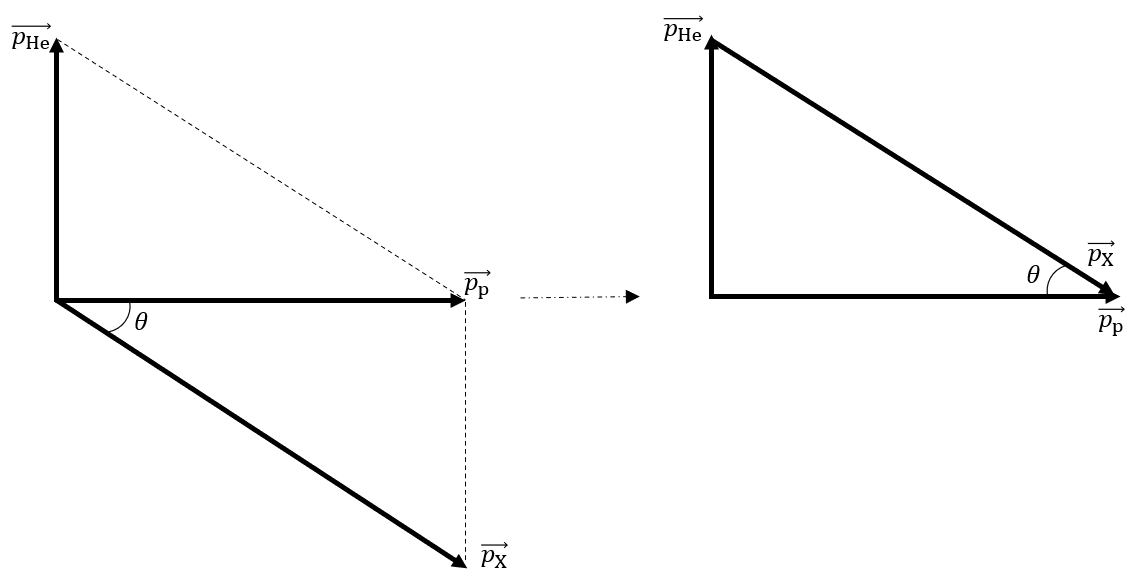
\includegraphics[scale=0.8]{../figs/VN12-2021-PH-TP037-3}
	\end{center}
	
	Áp dụng định lý Py-ta-go:
	$$p_{\ce{X}}^2 = p_{\ce{He}}^2 + p_{\ce{p}}^2$$
	
	Với $p^2=2mK$, ta được:
	$$2 m_{\ce{X}} K_{\ce{X}} = 2 m_{\ce{He}} K_{\ce{He}} +  2 m_{\ce{p}} K_{\ce{p}} $$
	
	Giải phương trình, tìm được:
	$$K_{\ce{X}} = \SI{3.57}{MeV}$$
		
	}
	
	\item \mkstar{2} [7]
	
	\cauhoi
	{Cho phản ứng hạt nhân sau:
		$$\ce{^9_4 Be} + \ce{p} \longrightarrow \ce{X} + \ce{^6_3 Li}$$
		
		Biết $m_{\ce{Be}} = \SI{9.01219}{u}$, $m_{\ce{p}} = \SI{1.00783}{u}$, $m_{\ce{X}} = \SI{4.00620}{u}$, $m_{\ce{Li}} = \SI{6.01515}{u}$, $\SI{1}{u} = \SI{931}{MeV/c^2}$. Cho hạt $\ce{p}$ có động năng $K_{\ce{p}} = \SI{5.45}{MeV}$ bắn phá hạt nhân $\ce{Be}$ đứng yên, hạt nhân $\ce{Li}$ bay ra với động năng $\SI{3.55}{MeV}$. Động năng của hạt $\ce{X}$ bay ra có giá trị là
		\begin{mcq}(4)
			\item $\SI{0.66}{MeV}$.
			\item $\SI{0.66}{eV}$.
			\item $\SI{66}{MeV}$.
			\item $\SI{660}{eV}$.
		\end{mcq}
	}
	
	\loigiai
	{		\textbf{Đáp án: A.}
		
		Năng lượng tỏa ra hoặc thu vào của phản ứng:
	$$Q=(m_\text{t} - m_\text{s})c^2 = \SI{-1.23823}{MeV}$$
	
	Lại có $Q=K_{\text{s}} - K_{\text{t}} = K_{\ce{X}} + K_{\ce{Li}} - K_{\ce{p}} \Rightarrow K_{\ce{X}} = \SI{0.66}{MeV}$
		
	}
	\item \mkstar{3} [1]
	
	\cauhoi
	{Người ta dùng hạt $\ce{\alpha}$ có động năng $K_{\ce{\alpha}}$ bắn vào hạt nhân nhôm $\ce{^27_13 Al}$ đứng yên gây ra phản ứng 
		$$\ce{^4_2 He} + \ce{^27_13 Al} \longrightarrow \ce{^30_15 P} + \ce{^1_0 n}$$
		Biết hạt nơtron và hạt nhân $\ce{^30_15 P}$ sinh ra sau phản ứng có động năng lần lượt là $\SI{1.8}{MeV}$ và $\SI{1}{MeV}$. Biết khối lượng của các hạt lần lượt là $m_{\ce{\alpha}} = \SI{4.00151}{u}$; $m_{\ce{Al}} = \SI{26.97435}{u}$; $m_{\ce{P}} = \SI{29.97005}{u}$; $m_{\ce{n}} = \SI{1.00867}{u}$. Động năng hạt $\ce{\alpha}$ là $K_{\ce{\alpha}}$ bằng
		\begin{mcq}(4)
			\item $\SI{5.464}{MeV}$.
			\item $\SI{4.232}{MeV}$.
			\item $\SI{5.644}{MeV}$.
			\item $\SI{4.328}{MeV}$.
		\end{mcq}
	}
	
	\loigiai
	{		\textbf{Đáp án: A.}
		
		Ta có năng lượng tỏa ra hoặc thu vào từ phản ứng là
	$$Q=(m_\text{t} - m_\text{s})c^2 = \SI{-2.66409}{MeV}$$
	
	Mà $Q=K_\text{s} - K_\text{t} \Rightarrow K_{\ce{P}} + K_{\ce{n}} - K_{\ce{\alpha}} - K_{\ce{Al}} = \SI{-2.66409}{MeV}$, suy ra $K_{\ce{\alpha}} = \SI{5.464}{MeV}$. (Chú ý rằng $K_{\ce{Al}}=0$ vì hạt nhân nhôm đứng yên)
	}
	\item \mkstar{3} [4]
	
	\cauhoi
	{Dùng một hạt $\ce{\alpha}$ có động năng $\SI{7.7}{MeV}$ bắn vào hạt nhân $\ce{^14_7 N}$ đang đứng yên gây ra phản ứng
		$$\ce{^4_2 He} + \ce{^14_7 N} \longrightarrow \ce{^1_1 p} + \ce{^17_8 O}$$
		Hạt proton bay ra theo phương vuông góc với phương bay tới của hạt $\ce{^4_2 He}$. Cho khối lượng các hạt nhân: $m_{\ce He} = \SI{4.0015}{u}$, $m_{\ce{N 14}} = \SI{13.9992}{u}$, $m_{\ce{O 17}} = \SI{16.9947}{u}$, $m_{\ce{p}} = \SI{1.0073}{u}$. Động năng của hạt nhân $\ce{^17_8 O}$ là
		\begin{mcq}(4)
			\item $\SI{2.075}{MeV}$.
			\item $\SI{2.214}{MeV}$.
			\item $\SI{6.145}{MeV}$.
			\item $\SI{1.345}{MeV}$.
		\end{mcq}
	}
	
	\loigiai
	{		\textbf{Đáp án: A.}
		
		
		Áp dụng định luật bảo toàn động lượng cho các hạt trước và sau phản ứng:
		$$\vec p_{\ce{\alpha}} = \vec p_{\ce{p}} + \vec p_{\ce{O}}$$
		
		Hình vẽ minh họa:
		\begin{center}
			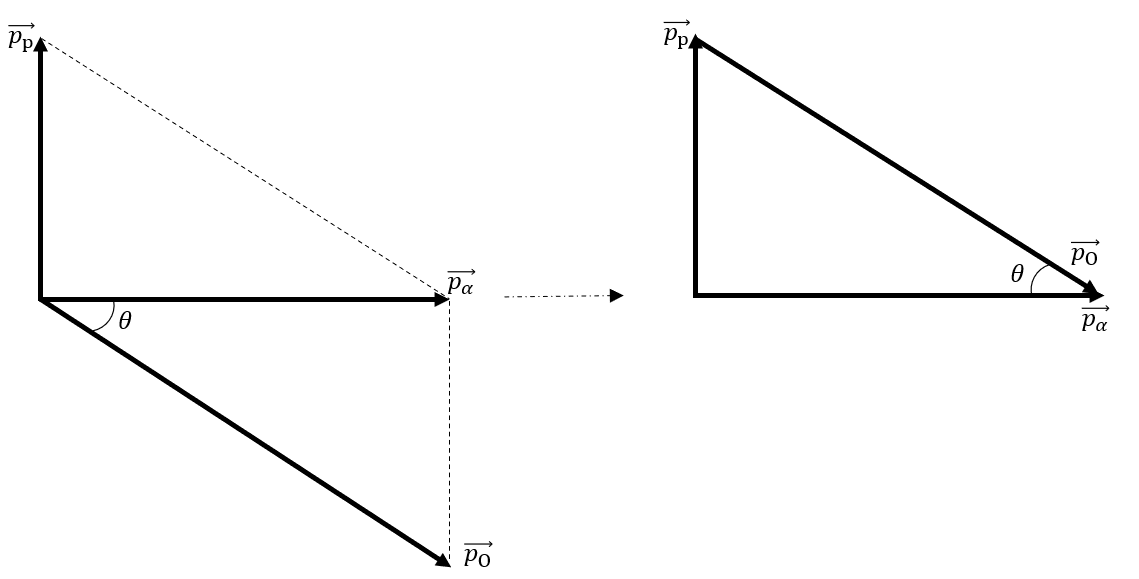
\includegraphics[scale=0.8]{../figs/VN12-2021-PH-TP037-2}
		\end{center}
		
		Áp dụng định lý Py-ta-go:
		$$p_{\ce{O}}^2 = p_{\ce{\alpha}}^2 + p_{\ce{p}}^2$$
		
		Với $p^2=2mK$, ta được:
		$$2 m_{\ce{O}} K_{\ce{O}} = 2 m_{\ce{\alpha}} K_{\ce{\alpha}} +  2 m_{\ce{p}} K_{\ce{p}} $$
		
		Kết hợp với công thức tính năng lượng tỏa ra hoặc thu vào:
		$$Q=(m_{\text{t}} - m_{\text{s}})c^2 = \SI{-1.21095}{MeV} = K_{\text s} - K_{\text t} = K_{\ce{p}} + K_{\ce{O}} - K_{\ce{He}}$$
		
		Giải hệ 2 phương trình, tìm được:
		$K_{\ce{p}} = \SI{4.417}{MeV}$ và $K_{\ce{O}} = \SI{2.072}{MeV}$
		
		Động năng của hạt nhân $\ce{^17_8 O}$ là xấp xỉ $\SI{2.075}{MeV}$.
	}
	\item \mkstar{3} [12]
	
	\cauhoi
	{Hạt nhân $\ce{^222_86 Rn}$ phóng xạ $\alpha$ tạo thành hạt nhân X. Ban đầu, hạt nhân $\ce{^222_86 Rn}$ đứng yên. Khối lượng mỗi hạt nhân bằng số khối của nó (đơn vị u). Ngay sau khi tạo thành, hạt $\ce{\alpha}$ và hạt X có tốc độ lần lượt là $v_1=\SI{2e7}{m/s}$ và $v_2$. Giá trị của $v_2$ xấp xỉ bằng
		\begin{mcq}(2)
			\item $\SI{366.972e3}{m/s}$.
			\item $\SI{10.034e5}{m/s}$.
			\item $\SI{109.021e3}{m/s}$.
			\item $\SI{605.015e3}{m/s}$.
		\end{mcq}
	}
	
	\loigiai
	{		\textbf{Đáp án: A.}
		
		Phản ứng hạt nhân:
	$$\ce{^222_86 Rn} \longrightarrow \ce{^4_2 He} + \ce{^218_84 X}$$
	
	Áp dụng định luật bảo toàn động lượng cho các hạt trước và sau phản ứng:
	$$\vec p_{\ce{Rn}} = \vec p_{\ce{\alpha}} + \vec p_{\ce{X}}$$
	
	Do $\vec p_{\ce{Rn}} = 0$ nên $\vec p_{\ce{\alpha}} + \vec p_{\ce{X}}$, suy ra:
	$$p_{\ce{\alpha}} = p_{\ce{X}}$$
	
	Với $p=\sqrt{2mK}$, và $\SI{1}{u} = \SI{1.6605e-27}{kg}$ ta được:
	$$2 m_{\ce{\alpha}} K_{\ce{\alpha}} = 2 m_{\ce{X}} K_{\ce{X}} \Rightarrow v_{\ce{X}} = \SI{366.972e3}{m/s}$$
	}
	\item \mkstar{4} [2]
	
	\cauhoi
	{Bắn một hạt proton có khối lượng $m_{\ce{H}}$ vào hạt nhân $\ce{^7_3 Li}$ đứng yên. Phản ứng tạo ra hai hạt nhân X giống nhau bay ra với vận tốc có cùng độ lớn và có phương vuông góc với nhau. Nếu xem gần đúng khối lượng hạt nhân theo đơn vị u bằng số khối của nó thì tỉ số tốc độ $v'$ của hạt X và $v$ của hạt proton là
		\begin{mcq}(4)
			\item $\dfrac{v'}{v} = \dfrac{1}{4}$.
			\item $\dfrac{v'}{v} = \dfrac{\sqrt{2}}{4}$.
			\item $\dfrac{v'}{v} = \dfrac{\sqrt 2}{8}$.
			\item $\dfrac{v'}{v} = \dfrac{1}{2}$.
		\end{mcq}
	}
	
	\loigiai
	{		\textbf{Đáp án: C.}
		
		Áp dụng định luật bảo toàn động lượng cho các hạt trước và sau phản ứng:
$$\vec p_{\text t} = \vec p_{\text s} \Rightarrow p_{\ce{p}}^2 = p_{\ce{X}}^2 + p_{\ce{X}}^2 = 2p_{\ce{X}}^2$$

Mà theo liên hệ $p^2=2mK$, suy ra:
$$2 m_{\ce{p}} K_{\ce{p}} = 2 \cdot 2 m_{\ce{X}} K_{\ce{X}} \Rightarrow m_{\ce{p}} K_{\ce{p}} = 2 m_{\ce{X}} K_{\ce{X}}$$

Thay $K=\dfrac{1}{2} mv^2$, ta được:
$$m_{\ce{p}} \cdot \dfrac{1}{2} m_{\ce{p}} v_{\ce{p}}^2 = 2 m_{\ce{X}} \cdot \dfrac{1}{2} m_{\ce{X}} v_{\ce{X}}^2 \Rightarrow \dfrac{v_{\ce{X}}^2}{v_{\ce{p}}^2} = \dfrac{m_{\ce{p}}^2}{2 m_{\ce{X}}^2} = \dfrac{1^2}{2 \cdot 4^2} = \dfrac{1}{32} \Rightarrow \dfrac{v'}{v} = \sqrt{\dfrac{1}{32}} = \dfrac{\sqrt 2}{8}$$
		
	}
	
	\item \mkstar{4} [3]
	
	\cauhoi
	{Bắn hạt nơtron có động năng $\SI{2}{MeV}$ vào hạt nhân $\ce{^6_3 Li}$ đứng yên gây ra phản ứng
		$$\ce{^1_0 n} + \ce{^6_3 Li} \longrightarrow \ce{X} + \ce{\alpha}.$$
		Hạt $\ce{\alpha}$ và hạt nhân $\ce{X}$ bay ra theo các hướng hợp với hướng tới của nơtron những góc tương ứng bằng $\theta = 15^\circ$ và $\varphi = 30^\circ$. Lấy tỉ số giữa các khối lượng hạt nhân bằng tỉ số giữa các số khối của chúng. Bỏ qua bức xạ gamma. Năng lượng của phản ứng hạt nhân \textbf{gần với giá trị nào nhất?}
		\begin{mcq}(4)
			\item Tỏa $\SI{1.52}{MeV}$.
			\item Thu $\SI{1.66}{MeV}$. 
			\item Thu $\SI{1.52}{MeV}$.
			\item Tỏa $\SI{1.66}{MeV}$.
		\end{mcq}
	}
	
	\loigiai
	{		\textbf{Đáp án: B.}
		
		Áp dụng định luật bảo toàn động lượng cho các hạt trước và sau phản ứng:
	$$\vec p_{\ce{n}} = \vec p_{\ce{X}} + \vec p_{\ce{\alpha}}$$
	
	Hình vẽ minh họa:
	\begin{center}
		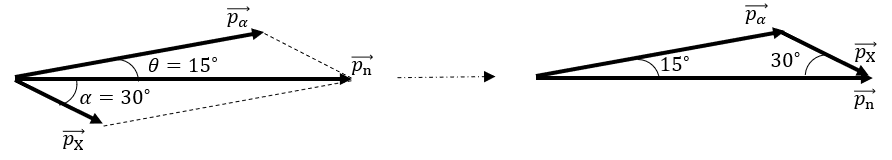
\includegraphics{../figs/VN12-2021-PH-TP037-1}
	\end{center}
	
	Áp dụng định lý hàm số sin:
	$$\dfrac{p_{\ce{n}}}{\sin 135^\circ} = \dfrac{p_{\ce{\alpha}}}{\sin 30^\circ} = \dfrac{p_{\ce{X}}}{\sin 15^\circ}$$
	
	Với $p=\sqrt{2mK}$, ta được:
	$$\dfrac{p_{\ce{n}}}{\sin 135^\circ} = \dfrac{p_{\ce{\alpha}}}{\sin 30^\circ} \Rightarrow \dfrac{\sqrt{2 m_{\ce{n}} K_{\ce{n}}}}{\sin 135^\circ} = \dfrac{\sqrt{2 m_{\ce{\alpha}} K_{\ce{\alpha}}}}{\sin 30^\circ}\Rightarrow K_{\ce{\alpha}} = \SI{0.25}{MeV} $$
	
	$$\dfrac{p_{\ce{n}}}{\sin 135^\circ} = \dfrac{p_{\ce{X}}}{\sin 15^\circ} \Rightarrow \dfrac{\sqrt{2 m_{\ce{n}} K_{\ce{n}}}}{\sin 135^\circ} = \dfrac{\sqrt{2 m_{\ce{X}} K_{\ce{X}}}}{\sin 15^\circ}\Rightarrow K_{\ce{X}} = \SI{0.09}{MeV} $$
	
	Năng lượng tỏa ra hoặc thu vào:
	$$Q=K_{\text{s}} - K_{\text{t}} = \SI{-1.66}{MeV}$$
	
	Do $Q<0$ nên phản ứng thu năng lượng.
	}
	
	
	
	
	
	
\end{enumerate}

\loigiai
{
	\begin{center}
		\textbf{BẢNG ĐÁP ÁN}
	\end{center}
	\begin{center}
		\begin{tabular}{|m{2.8em}|m{2.8em}|m{2.8em}|m{2.8em}|m{2.8em}|m{2.8em}|m{2.8em}|m{2.8em}|m{2.8em}|m{2.8em}|}
			\hline
			1.D  & 2.A  & 3.A  & 4.A  & 5.A  & 6.A  & 7.A & 8.C & 9.B & \\
			\hline
			
		\end{tabular}
	\end{center}
}

\whiteBGstarEnd